% Template for ICASSP-2019 paper; to be used with:
%          spconf.sty  - ICASSP/ICIP LaTeX style file, and
%          IEEEbib.bst - IEEE bibliography style file.
% --------------------------------------------------------------------------
\documentclass{article}
\usepackage{spconf,amsmath,graphicx,multirow}

% Example definitions.
% --------------------
\def\x{{\mathbf x}}
\def\L{{\cal L}}

% Title.
% ------
\title{Saliency Map on CNNs for Protein Secondary Structure	Prediction}
%
% Single address.
% ---------------
\name{Guillermo Romero Moreno \qquad Mahesan Niranjan \qquad Adam Prugel-Bennett}%\thanks{Thanks to XYZ agency for funding.}}
\address{School of Electronics and Computer Science\\
	University of Southampton, Southampton, UK\\
	Email: grm1g17@soton.ac.uk, m.niranjan@southampton.ac.uk, apb@ecs.soton.ac.uk}
%
% For example:
% ------------
%\address{School\\
%	Department\\
%	Address}
%
% Two addresses (uncomment and modify for two-address case).
% ----------------------------------------------------------
%\twoauthors
%  {A. Author-one, B. Author-two\sthanks{Thanks to XYZ agency for funding.}}
%	{School A-B\\
%	Department A-B\\
%	Address A-B}
%  {C. Author-three, D. Author-four\sthanks{The fourth author performed the work
%	while at ...}}
%	{School C-D\\
%	Department C-D\\
%	Address C-D}
%
\begin{document}
%\ninept
%
\maketitle
%
\begin{abstract}
%The abstract should appear at the top of the left-hand column of text, about
%0.5 inch (12 mm) below the title area and no more than 3.125 inches (80 mm) in
%length.  Leave a 0.5 inch (12 mm) space between the end of the abstract and the
%beginning of the main text.  The abstract should contain about 100 to 150
%words, and should be identical to the abstract text submitted electronically
%along with the paper cover sheet.  All manuscripts must be in English, printed
%in black ink.

Deep learning has been successfully transferred to the biomedical field, achieving higher performance but bringing opaqueness. While interpretability techniques are under current development, only a few authors have brought them to the biomedical field. This work aims to apply one of such techniques ---saliency maps--- in the context of protein secondary structure prediction. For doing so, a convolutional neural network was first trained, saliency maps obtained from it, and different ways of aggregating them have been developed to gather meaningful insights on the network's learning of the underlying problem structure. The analysis of saliency maps led to interesting findings, namely the irrelevance of one-hot amino-acid inputs and the higher importance of right positions for the prediction of $\alpha$-helices. These techniques can be of double value: they help biologists to get a better understanding of the underlying processes and machine learning researchers can spot previously uncovered flaws.
\end{abstract}
%
\begin{keywords}
Saliency Maps, Convolutional Neural Networks, Protein Secondary Structure Prediction, Interpretability.
\end{keywords}
%
\section{Introduction}
\label{sec:intro}

%TAlk about deep learning and its inclusion into biology studies

%INclude many references

Secondary structure prediction is a long-time studied problem in bioinformatics. The 3D structure of a protein determines the function it is going adopt in the cell. However, the protein structure cannot be easily measured and any attempt to do so remains costly. A more feasible alternative is utilising computational tools to make the predictions having as a base the amino-acid sequence (easy to obtain through DNA sequencing) and the proteins whose structure is already known. Predicting the secondary structure is often regarded as a middle step for tackling the much harder problem of predicting the 3D structure. The protein secondary structure prediction problem is a sequence structural tagging problem: each element (amino-acid) of the protein sequence has to be assigned a class (secondary structure). There are 21 different types of amino-acids and eight possible goal classes, which are composed of 3 types of helices(H, G, I), two types of $\beta$-sheets (B, E), and three types of coils (T, S, L)~\cite{Kabsch1983}. Other relevant features of the amino-acids can also be added as inputs to facilitate the classification process. A common one whose addition brought a significant performance improvement is the Position Specific Substitution Matrices (PSSM)~\cite{Yang2018}, which encode the evolutionary probability of finding substitutions in each element of the amino-acid chain. The final input sequence would have length \textit{l} (variable from protein to protein) and width 42: the one-hot encoded amino-acid plus the 21 extra values of the PSSM, normalized to a range between zero and one~\cite{Busia2017}. While at the early stages the secondary structure prediction problem was mainly tackled with statistics, towards the end of the century the application of neural networks became prevalent \cite{Rost1993}. A new generation of deep learning approaches started recently with~\cite{Zhou2014}, who implemented a Generative Stochastic Network fed by a 1D Convolutional Neural Network (CNN) architecture, and later works that already included 1D CNNs with five or more layers~\cite{Fang2017,Zhou2018} or recurrent neural networks~\cite{Li2016,Jurtz2017}, which are deep in the sense of signals being processed for many time-steps.

Saliency maps are a visualisation technique for sensitivity analysis. A saliency map has the same dimensions as the input and contains their importance values, e.g. their contribution to the output. Depending on their calculation method, saliency maps can be broadly grouped into \textit{perturbation-based approaches} (make modifications on the input and assess changes in the output) or \textit{backpropagation-based approaches} (utilise the gradient of the output respect to the input for obtaining the importance information)~\cite{Shrikumar2017}. Although the first group is intuitive and useful for small input spaces, it becomes quickly intractable when the input size grows, as all possible combinations of inputs should be examined for a complete analysis. The second group ---especially designed for neural networks--- allows the computation of importance scores in a single backward pass, so its computational complexity significantly improves and hence it is the preferred option for such architectures.

Back-propagation approaches can be thought as a linear approximation of the classification function around a sample input point $x_0$ by applying a first-order Taylor expansion, as introduced in~\cite{Simonyan2014}:
\begin{align}
f(x) \approx w^T x + b \; , \\
w = \left. \frac{\partial f}{\partial x} \right|_{x_0} \; .
\end{align}
In their simplest form, the saliency maps of back-propagation methods are equivalent to the gradient value on the input \cite{Simonyan2014}. A second approach~\cite{Bach2015} would multiply the gradient by the input values to leverage out the gradients that don't carry relevant information. A last wave of methods proposes including a reference point and hence more closely resembling the Taylor approximation. The main examples of this trend are integrated gradients~\cite{Sundararajan2017}, deep Taylor decomposition~\cite{Montavon2017} and DeepLIFT~\cite{Shrikumar2017}. They overcome problems of previous methods such as saturation or discontinuities in the gradient, although they bring the extra difficulty of choosing an appropriate reference point.

\section{Previous work}
\label{sec:prevwork}

%The text of the paper should contain discussions on how the paper's
%contributions are related to prior work in the field. It is important
%to put new work in context, to give credit to foundational work, and
%to provide details associated with the previous work that have appeared
%in the literature. This discussion may be a separate, numbered section
%or it may appear elsewhere in the body of the manuscript, but it must
%be present.
%
%You should differentiate what is new and how your work expands on
%or takes a different path from the prior studies. An example might
%read something to the effect: "The work presented here has focused
%on the formulation of the ABC algorithm, which takes advantage of
%non-uniform time-frequency domain analysis of data. The work by
%Smith and Cohen \cite{Lamp86} considers only fixed time-domain analysis and
%the work by Jones et al \cite{C2} takes a different approach based on
%fixed frequency partitioning. While the present study is related
%to recent approaches in time-frequency analysis [3-5], it capitalizes
%on a new feature space, which was not considered in these earlier
%studies."

%As a simplified version of saliency maps, Alipanahhi et al.~\cite{Alipanahi2015} and Quang and Xie~\cite{Quang2016} spotted the segment in the input genetic sequence that had the highest activation of the first-layer filters and compared them to known motifs. This approach only makes sense as long as the network has a single layer, but cannot be applied to deeper networks.

Perturbation-based approaches are prevalent, with perturbation as genetic mutations~\cite{Alipanahi2015,Zhou2015}, small sliding windows with random genetic code~\cite{Umarov2017} or known motifs~\cite{Kelley2016}, among others. Gradient-based approaches have barely been translated to the biological field. Lanchantin et al.~\cite{Lanchantin2016} include saliency maps with the form of gradient $\times$ input for TF binding site classification. They extracted the window with the highest score from each saliency map and compared them with a database of known motifs, matching almost half of the motifs thus produced. Shrikumar et al.~\cite{Shrikumar2017} developed the reference-based saliency map technique DeepLIFT and simulated a motif detection task within a genomic sequence to prove its effectiveness. Finnegan and Song~\cite{Finnegan2017} utilised Markov chain Monte Carlo methods to withdraw samples from the maximum entropy distribution around a single sequence and assessed the importance scores by looking at the variance of the samples at each position. This method was applied to a previously trained DNA-protein binding CNN and proved to have better results than DeepLIFT.

All these methods address classification problems where there is a single output (classification task) for each sequence. A significant difference between this work and previous papers that make use of saliency maps is that they focus on many-to-one classification problems (one output class per input sequence/image), whereas our classification task is many-to-many (each position of the sequences is assigned a class), producing as many saliency maps as positions in a sequence. To the best of our knowledge, interpretability techniques have not been applied yet to this sort of problems.

\section{Methods}
\label{sec:methods}

The experiments used the database produced and made public by Zhou and Troyanskaya~\cite{Zhou2014}. It includes two sub-sets (training and test, with 5534 and 514 protein sequences of varying length, respectively) of proteins that come from different sources after removing the proteins that share 25\% or more similarity, thus ensuring that the test set is composed of totally new samples. The proteins in the dataset already come in one-hot form, along with their Q8 class in one-hot as well and PSSM values. The dataset is heavily imbalanced, as it can be seen in Table \ref{table:q8}

\begin{table}
	\begin{tabular}{cc|c|c}
		\multicolumn{2}{c}{\textbf{Q8 grouping}} &  \textbf{Explanation} & \textbf{\%}\\ 
		$\alpha$-helix & H & Helix with 4 turns & 34.54 \\ 
		$3_{10}$-helix & G & Smaller helix with 3 turns & 3.91 \\ 
		$pi$-helix      & I & Bigger helix with 5 turns & 0.02 \\ \hline
		$\beta$-bridge & B & Isolated $\beta$-bridge & 1.03 \\ 
		$\beta$-strand & E & Participates in $\beta$-ladders & 21.78\\ \hline
		Turn & T & Turns smaller than a helix & 11.28 \\ 
		Bend & S & Curved piece & 8.26 \\ 
		Loop & L & Sometimes also as coil (C) & 19.19
	\end{tabular}
	\caption{Targets for the secondary structure prediction problem, as defined by Kabsch and Sander~\cite{Kabsch1983} in their Dictionary of Secondary Structure or Proteins (DSSP) and their presence on the training set.}
	\label{table:q8}
\end{table}

The network architecture is composed of three successive convolutional neural networks and a dense layer on top. Each of the convolutional layers contains three sets of filters of size 3, 5 and 7, respectively, with 16 filters per size. There are skip connections at every convolutional layer. The dense layer has 200 neurons and is connected to the softmax output layer. The convolution operations are carried out with padding at each end of the sequence to preserve the length throughout the process. The total window size of the network is 19, meaning that for making a single secondary structure classification the network obtains information from 9 adjacent positions at each side. The network has been built and trained using the open-source code developed by Jurtz et al.~\cite{Jurtz2017}.

Saliency maps are calculated by the conventional technique of computing the gradient of the output with respect to the inputs and multiplying it by the value of the input (gradient $\times$ input)~\cite{Shrikumar2016}. Every single position in a sequence produces a saliency map that spans the width of the input vector of size 42 and 9 positions to each side, due to the architecture's window size of 19. Each output class has its independent saliency values, so the total size of a position saliency map is 8x42x19.

The presence of overlapping saliency maps allows for different ways in which to aggregate them to extract meaningful information. If we focus on a sequence of length $l$ and want to obtain a single sequence-specific saliency map, we can add up the overlapping areas to form a saliency map of size 8x42x$l$. By changing the focus to a broader look on what the network has learnt, the addition of the saliency maps for the positions in all sequences could create a single saliency map of size 8x42x19 that shows an average behaviour of the network. From this map, we can extract general information about a particular class (creating a class-specific saliency map) or about a particular input (PSSM-specific saliency map).

\section{Results}
\label{sec:results}

The network described in the previous section has been trained for 400 epochs with regularisation parameter $\lambda=10^{-4}$, and learning rate $\mu=10^{-4}$. Five of such networks with different weight initialisation are trained, and the set of weights for each of them with highest validation accuracy\footnote{On a validation subset of the training set, with 512 sequences.} is taken to form an ensemble that reaches an accuracy of $69.23\%$ on the test set, not far from the $71\%$ reached by the state-of-the-art~\cite{Busia2017}. The aim of this work is not to outperform the state-of-the-art predictions, but to build a network with a moderately simple structure (to keep the calculation times of saliency maps on reasonable levels) and fair performance. We believe that the techniques of analysis here presented and the conclusions withdrawn from them can be transferred to current state-of-the-art methods without losing validity.
\begin{figure}[t]
	\centering
	\centerline{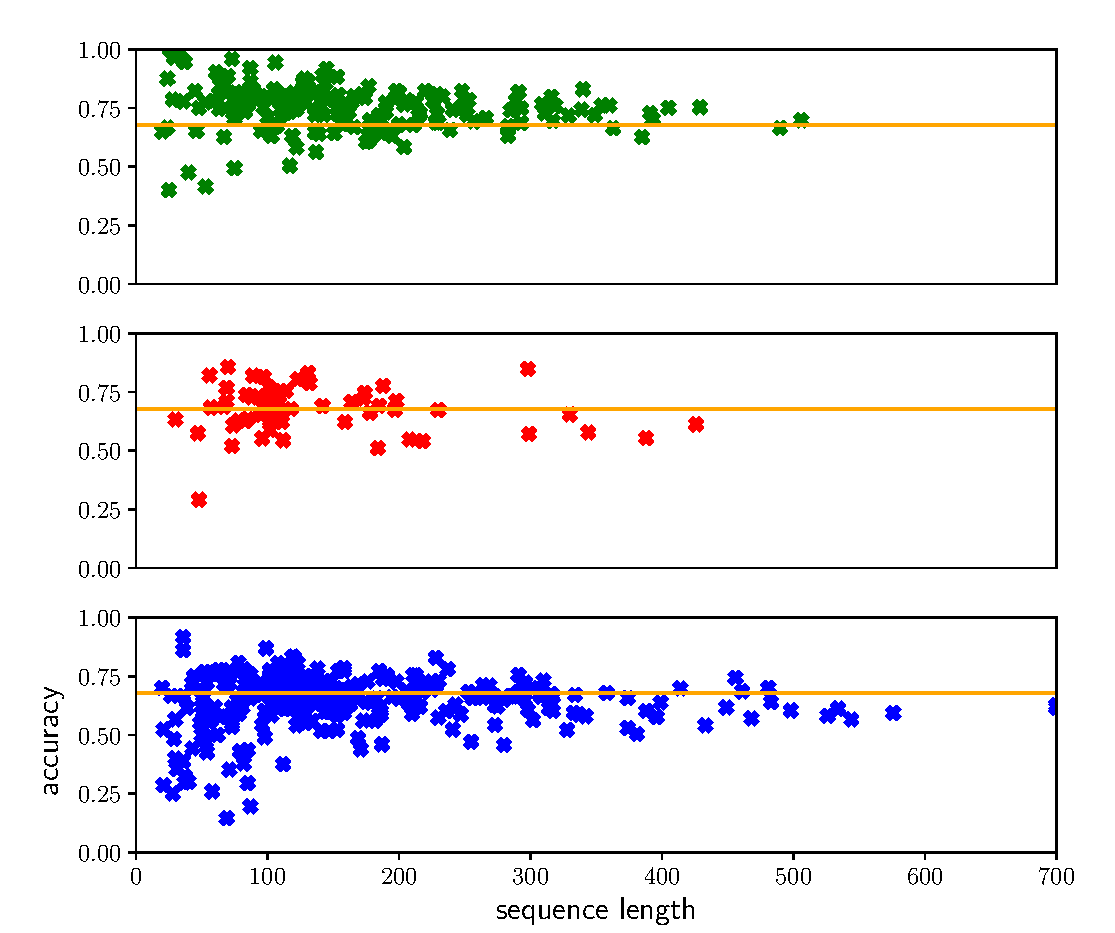
\includegraphics[width=8.6cm]{per_seq_acc}}
	%  \vspace{1.5cm}
	\caption{Mean sequence accuracy against sequence length for the proteins in test set. Each point represents a single protein sequence and the horizontal line is the total mean accuracy. On top, sequences with majority of helices (H, G, I); $\beta$-sheets (E, B) at the middle; and coils (L, S, T) below. Best accuracies are achieved with high percentage of helices and worst accuracies with with majority of coils.}
	\label{fig:accuracies}
	%
\end{figure}

Figures \ref{fig:accuracies} and \ref{fig:confusion} show more information on the network performance. Figure \ref{fig:accuracies} shows the distribution of per-sequence accuracies over different sizes.
As it could be expected, the variance in mean accuracy increases with shorter sequences. Higher accuracies can be expected from sequences rich in helices and lower accuracies for sequences high in coils. Figure \ref{fig:confusion} displays the resulting confusion matrix of the predictions on the test set.
\begin{figure}[t]
	\centering
	\centerline{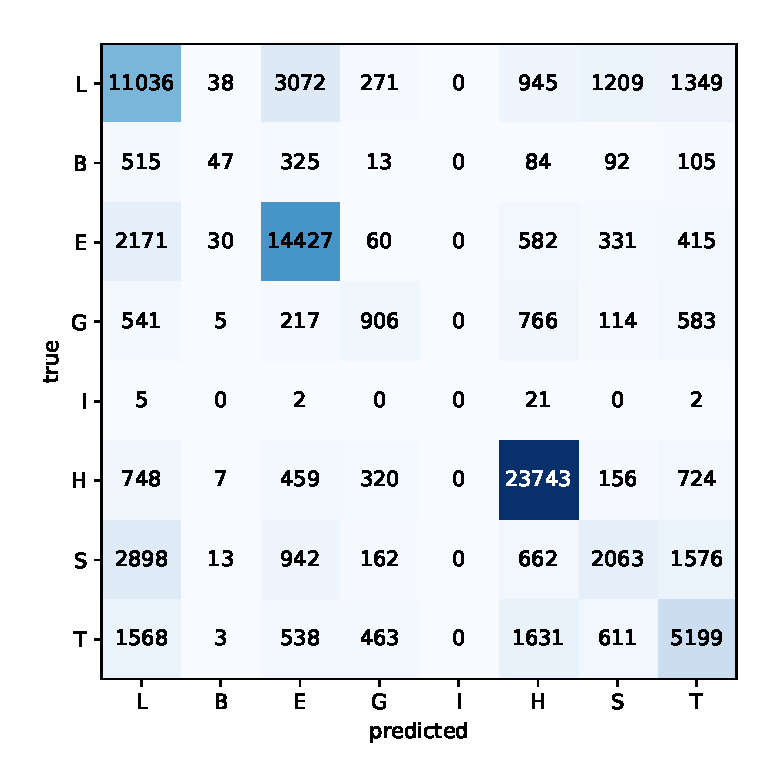
\includegraphics[width=7.5cm]{confusion}}
	%  \vspace{1.5cm}
	\caption{Confusion matrix of the test set. Classes I and B are scarce in the dataset; classes G, H and T have relatively high levels of confusion because they are all composed of turns, but with different lengths; loops (L) are a loose category and their confusion is also high.}
	\label{fig:confusion}
	%
\end{figure}
It is similar to the ones obtained on other state-of-the-art networks~\cite{Fang2017}. It is noticeable that the $\pi$-helix (I) has never been given as prediction; its presence is so rare in the dataset that the machine keeps a higher accuracy by ignoring it. $\beta$-bridges (B) are also largely misrepresented for the same reasons. Loops present high levels of confusion with other classes, probably due to the arbitrary discretisation into eight classes, while it has been pointed that it is not that clear the class assignation at the transitions between structures and coils~\cite{Rost2001}.

Saliency maps can be used as additional evidence for theories around protein secondary structure. For instance, one point of concern has been the inclusion of inputs with different nature: the one-hot amino-acid along the PSSM dense vector. Some authors \cite{Li2016,Zhou2018} embedded the one-hot vector into a denser space, reporting a small marginal improvement in accuracy (0.5\% and 0.4\%, respectively). Spencer et al.~\cite{Spencer2015} reported a 2\% Q3 improvement by not including the one-hot amino-acids at all. Saliency maps provide information of about the importance that different parts of the input have, so direct comparison of both kinds of inputs can be made by looking at their associated saliency values. To do so, each saliency map is split into two halves, corresponding to amino-acid and PSSM, respectively, and all the values of each half are summed up in absolute value to form a single saliency score. The comparison of such scores for all positions in the dataset is made in Figure \ref{fig:aa_pssm}, revealing that in the great majority of positions the PSSM inputs had four times or more relevance for making the classification decision, with around half of them having seven times or more relevance.
\begin{figure}
	\centering
	\centerline{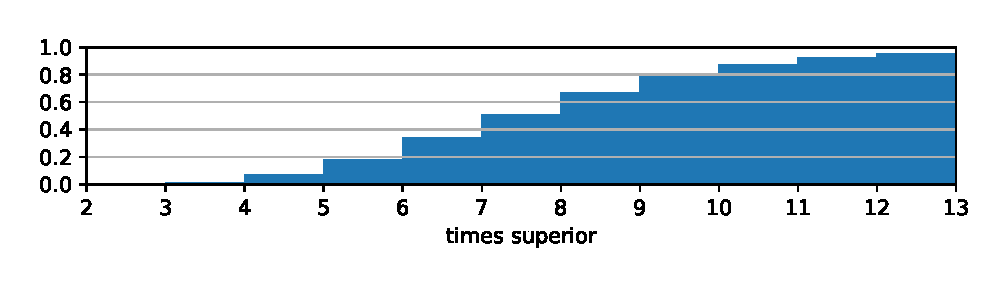
\includegraphics[width=8.6cm]{aa_pssm}}
	%  \vspace{1.5cm}
	\caption{Cumulative histogram of how much bigger are PSSM saliency scores as compared to aminoa-acid saliency scores.}
	\label{fig:aa_pssm}
	%
\end{figure}
We further validate these findings by training a second network that uses PSSM inputs but ignores the one-hot amino-acids, all the other things remaining equal. An ensemble of five of these networks reaches an accuracy of $69.36\%$ on the test set, $0.14\%$ points higher than the original configuration (see Table \ref{table:res}).
\begin{table}
	\centering
	\begin{tabular}{c|c|c}
		\textbf{Labels} 	& \textbf{Architecture} & \textbf{Accuracy} \\
		\multirow{2}{*}{Q8} & Original 			& 69.23\% \\
		& PSSM-only 		& \textbf{69.36}\% \\ \hline
		\multirow{2}{*}{H / non-H} & Right positions only & \textbf{86.60}\% \\
		& Left positions only & 80.81\%
	\end{tabular}
	\caption{Accuracies on the test set for different network configurations. Ensembles of networks performed better by ignoring one-hot amino-acids. Networks that look on a window of size nine at the right side predict class H better than when they regard the nine left positions.}
	\label{table:res}
\end{table}

Another useful application of saliency maps can be the study of spatial importance around the predicted position. Figure \ref{fig:sheereq} includes the average saliency spatial profiles for each class.
\begin{figure}[t]
	\centering
	\centerline{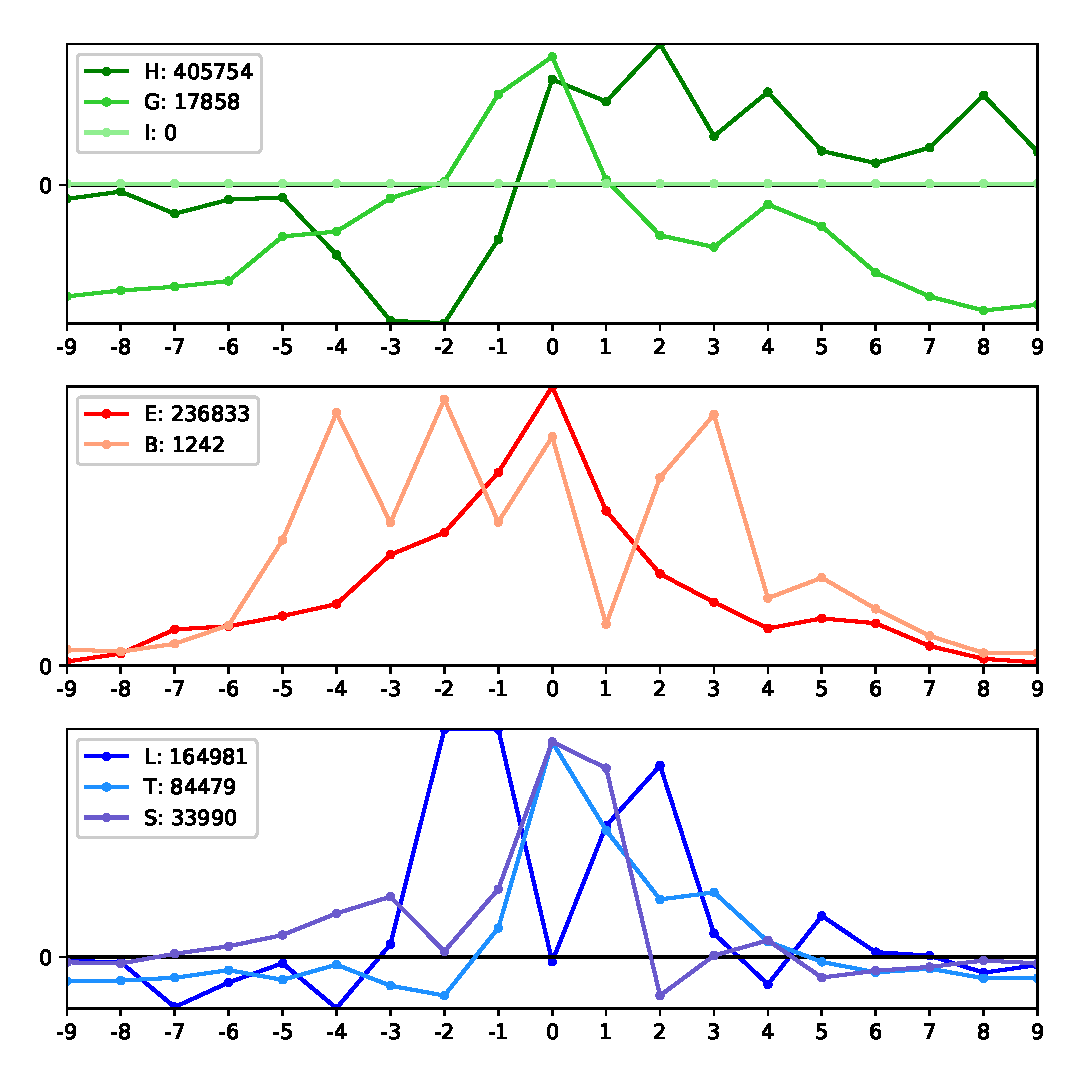
\includegraphics[width=8.6cm]{sheerabsequal6016_class_aa}}
	%  \vspace{1.5cm}
	\caption{Average saliency profiles for the eight classes. On top, the three helix classes; in the middle, the two $\beta$ classes; below, the three coil classes. The legends show the number of profiles averaged over for each class. We want to focus on the distribution of each class over the window positions, so each line has been independently normalized for a clearer visualisation of each shape and scales only shared the zero reference.}
	\label{fig:sheereq}
	%
\end{figure}
The construction of each profile has been made as follows. For each sequence position belonging to the class that was predicted right, the 42x19 slice of the saliency map corresponding to the class is extracted and summed up over the feature dimensions, leading to a profile vector of size 19. The figure shows the average of all of such profiles for each class. Sequences coming from both the training and test set were used for this result. The profiles reveal what the spatial influence for each class. For instance, the $\alpha$-helices (H) hold some periodicity at the right side and large asymmetry. The periodicity could go in line with the structure of helices, which are a succession of turns. The asymmetry can point to a strong dependency on posterior amino-acids when the protein chain is built instead of what was coming before. To validate this finding, we re-train two new networks for binary classification of H / non-H. The networks have an identical structure to the previous ones with the only modification being that one of them ignores the input from the left positions and the other the ones from the right positions\footnote{This is achieved by zeroing out different halves of the parameters on the convolutional filters.}. While the network making use of the left positions obtains an accuracy of $80.81\%$ on the test set, the one utilising the right positions achieves $86.60\%$, supporting the idea that future positions are more significant in the formation of an $\alpha$-helix (Table \ref{table:res}).

%Figure~\ref{fig:result} shows a fragment of a sequence-specific saliency map for one of the eight classes (H). It reveals which PSSM values in the vicinity are mostly responsible for the predictions of class H in the fragment. The real amino-acids that are in the sequence are not always as influential in the algorithm decisions as other of the PSSM values, which explains why the inclusion of the later significantly improves the performance of predictions. PSSM values for specific amino-acids do not need to have contributions of the same sign (such P or D reveal in the figure), so the network is capturing something more than pure presence of the PSSM values in the vicinity: their location and combination is also influential. The saliency maps can help to find significant motifs that give raise to specific secondary structures.

%\begin{figure*}
%	\centering
%	\centerline{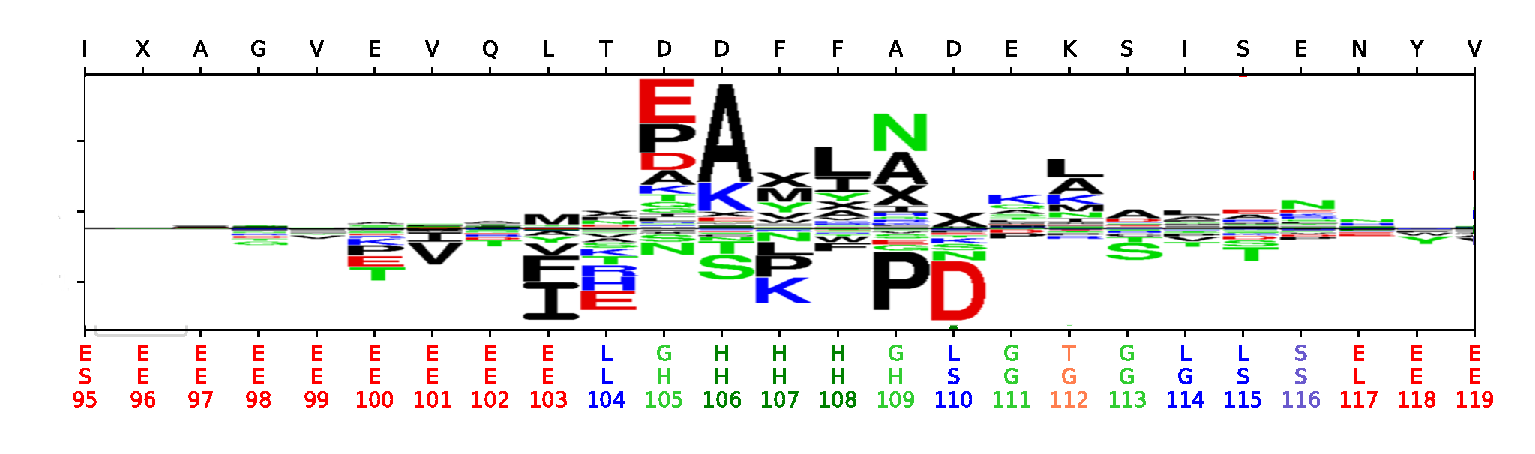
\includegraphics[width=17.8cm]{sample_Hclass}}
%	%  \vspace{1.5cm}
%	\caption{Fragment of a sequence-specific saliency map for class H in sequence logo form. Only the saliency of PSSM values is shown here. The upper x axis displays the amino-acids that form the sequence. The lower x axis contains three sets of labels: the predictions, the true values, and the position number in the sequence, respectively. The sequence logo has been generated by \textit{Seq2Logo}~\cite{Thomsen2012}.}
%	\label{fig:result}
	%
%\end{figure*}


\section{Conclusions}
\label{sec:conclusions}

Sensitive analysis help with dealing with the opaqueness of deep neural networks. Saliency maps are one of such techniques which have been extensively applied in the computer vision field but has barely been transferred to biomedical research. In this work, we have successfully applied saliency maps to the secondary structure prediction problem and shown that they can reveal insights from what the network has learnt, such as the irrelevance of one-hot amino-acid inputs or the strong dependence on future positions for the formation of $\alpha$-helices.

%\section{ILLUSTRATIONS, GRAPHS, AND PHOTOGRAPHS}
%\label{sec:illust}

%Illustrations must appear within the designated margins.  They may span the two
%columns.  If possible, position illustrations at the top of columns, rather
%than in the middle or at the bottom.  Caption and number every illustration.
%All halftone illustrations must be clear black and white prints.  Colors may be
%used, but they should be selected so as to be readable when printed on a
%black-only printer.

%Since there are many ways, often incompatible, of including images (e.g., with
%experimental results) in a LaTeX document, below is an example of how to do
%this \cite{Lamp86}.


% Below is an example of how to insert images. Delete the ``\vspace'' line,
% uncomment the preceding line ``\centerline...'' and replace ``imageX.ps''
% with a suitable PostScript file name.
% -------------------------------------------------------------------------
%\begin{figure}[htb]
%
%\begin{minipage}[b]{1.0\linewidth}
%  \centering
%  \centerline{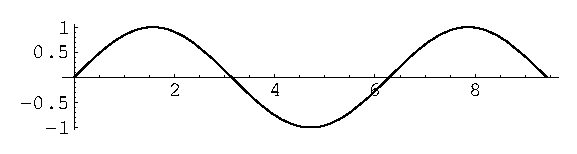
\includegraphics[width=8.5cm]{image1}}
%%  \vspace{2.0cm}
%  \centerline{(a) Result 1}\medskip
%\end{minipage}
%%
%\begin{minipage}[b]{.48\linewidth}
%  \centering
%  \centerline{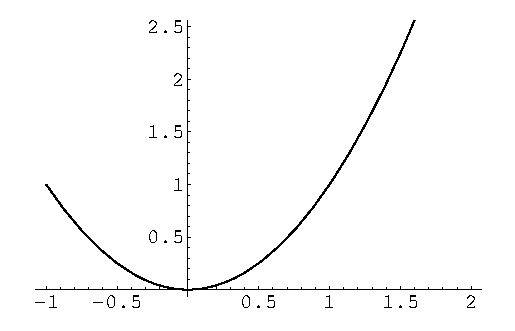
\includegraphics[width=4.0cm]{image3}}
%%  \vspace{1.5cm}
%  \centerline{(b) Results 3}\medskip
%\end{minipage}
%\hfill
%\begin{minipage}[b]{0.48\linewidth}
%  \centering
%  \centerline{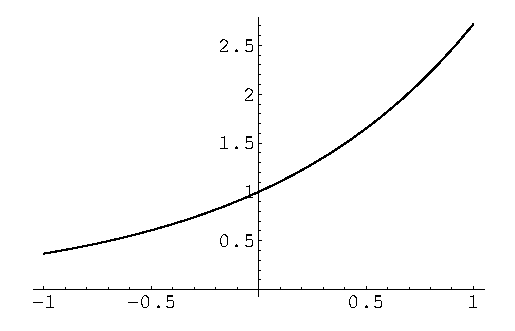
\includegraphics[width=4.0cm]{image4}}
%%  \vspace{1.5cm}
%  \centerline{(c) Result 4}\medskip
%\end{minipage}
%%
%\caption{Example of placing a figure with experimental results.}
%\label{fig:res}
%%
%\end{figure}


% To start a new column (but not a new page) and help balance the last-page
% column length use \vfill\pagebreak.
% -------------------------------------------------------------------------
%\vfill
%\pagebreak

%\section{COPYRIGHT FORMS}
%\label{sec:copyright}

%You must submit your fully completed, signed IEEE electronic copyright release
%form when you submit your paper. We {\bf must} have this form before your paper
%can be published in the proceedings.

\vfill\pagebreak

% References should be produced using the bibtex program from suitable
% BiBTeX files (here: strings, refs, manuals). The IEEEbib.bst bibliography
% style file from IEEE produces unsorted bibliography list.
% -------------------------------------------------------------------------
\bibliographystyle{IEEEbib}
\bibliography{refs}

\end{document}
